\section{Preliminaries}\label{sec:prelims}
In this section, we introduce the necessary terminology, concepts, and tools
that we will use to develop our results in the following sections.

\subsection{Databases and Queries}\label{sec:dbqueries}
We outline here some basic definitions about databases, queries, and
selectivity. We refer the reader to complete textbooks for additional
information~\citep{GarciaMolinaUW02}.
We consider a \emph{database} $\Db$ of $k$ tables $\Tab_1,\dotsc,\Tab_k$. 
A \emph{table} $\Tab$ is a two-dimensional representation of data. It
contains a number of rows or \emph{tuples}, and may (and typically does) have multiple
\emph{columns}. We denote a column $C$ of a table $\Tab$ as $\Tab.C$ and, for a
tuple $t\in\Tab$, the value of $t$ in the column $C$ as $t.C$. We denote the
domain of the values that can appear in a column $\Tab.C$ as $\domain{\Tab.C}$.
Each tuple $t$ is then an element from the Cartesian product of the domains of
the columns of $\Tab$, $t\in \domain{\Tab.C_1}\times\dotsb\times
\domain{\Tab.C_m}$. Figure~\ref{tab:example} shows two examples of database
tables, \emph{Customers} and \emph{CarColors}. 

\begin{figure}[htb]
  \begin{subtable}[b]{0.6\textwidth}
    \centering
    \begin{tabular}{c|c|c|c|c}
      %\toprule
      \multicolumn{5}{c}{\emph{Customers}} \\
      \midrule
      \emph{Name} & \emph{Age} & \emph{Street} & \emph{ZipCode} & \emph{CarBrand} \\
      \midrule
      \texttt{John Doe} & \texttt{20} & \texttt{Pratt Av.} & \texttt{02906} & \texttt{BMW} \\
      \texttt{Jim Clark} &  \texttt{30} &\texttt{Morris Rd.} & \texttt{02906} & \texttt{Lotus} \\
      \texttt{Greta Garbo} & \texttt{60} & \texttt{Pratt Av.} & \texttt{05902} & \texttt{Rolls-Royce} \\
      \bottomrule
    \end{tabular}
    \caption{A table with four columns}
  \end{subtable}
  \hfill
  \begin{subtable}[b]{0.3\textwidth}
    \centering
    \begin{tabular}{c|c}
      \multicolumn{2}{c}{\emph{CarColors}} \\
      \midrule
      \emph{Name} & \emph{Color} \\
      \midrule
      \texttt{John Doe} & \texttt{Black} \\
      \texttt{Jane Doe} & \texttt{Red} \\
      \texttt{Greta Garbo} & \texttt{Red}\\ 
      \bottomrule
    \end{tabular}
    \caption{A table with two columns}
  \end{subtable}
  \caption{Example of two database tables.}
  \label{tab:example}
\end{figure}

A \emph{query} $q$ is a function that takes as input one or more tables and
returns a set of elements the Cartesian product of the input tables. This set
depends on the database $\Db$ which the input tables to $q$ belong to, and we
denote with $\Out_\Db(q)$ and we call it the output of $q$ on $\Db$. The
\emph{cardinality} $\card_\Db(q)$ of $q$ on $\Db$ is the size
$|\Out_\Db(q)|$. The \emph{selectivity} $\selectivity_\Db(q)$ of $q$ on $\Db$ is
the ratio between $\card_\Db(q)$ and the \emph{product} of the sizes of the
input tables of $q$.  Clearly, $0\le\selectivity_\Db(q)\le 1$.

There are many different types of queries. We now introduce the ones we are interested
in for our purposes.
\begin{definition}\label{def:selectquery}
  Given a table $\Tab$ with columns $\Tab.C_1,\dotsc,\Tab.C_\ell$, a
  \emph{selection query} $q$ on $\Tab$ is a function which returns a subset
  $S$ of the tuples of $\Tab$ such that a tuple $t$ of $\Tab$ belongs to $S$ if
  and only if the values in $t$ satisfy a condition $\mathcal{C}$
  (the \emph{selection predicate}) expressed by $q$. In full
  generality, $\mathcal{C}$ is the Boolean combination of clauses of the form
  ``$\Tab.C_i \op a_i$'', where $\Tab.C_i$ is a column of $\Tab$, ``$\op$'' is one
  of $\{<,>,\ge,\le,=,\neq\}$ and $a_i$ is an element of the domain of
  $\Tab.C_i$.
\end{definition}

As an example, the selection query 
\[
\SELECT * \FROM \text{\emph{Customers}} \WHERE \text{\emph{Customers.ZipCode}} = 02906;
\]
would return the first and second row of Table~\ref{tab:example}.

\note{Maybe the following should go on top, rephrased.}
We assume that, for each column $\Tab_C$ of each table $\Tab$, the domain
$\domain{\Tab.C_i}$ is such that it is possible to build a total order relations
on it. This assumptions does not exclude categorical domains from our
discussion, because the only meaningful values for ``$\op$'' for such domains
are ``$=$'' and ``$\neq$'', so we can just assume an arbitrarily but fixed order
for the categories in the domain.

\begin{definition}\label{def:joinquery}
  Given two tables $\Tab_1$ and $\Tab_2$, a $\emph{join query}$ $q$ on a common
  column $C$ (i.e., a column present both in $\Tab_1$ and $\Tab_2$) is a
  function which returns a subset of the Cartesian product of the tuples in
  $\Tab_1$ and $\Tab_2$. The returned subset is defined as the set $ \{(t_1,t_2)
  ~:~ t_1\in\Tab_1, t_2\in\Tab_2, \text{ s.t. } t_1.C \op t_2.C \}$ where
  ``$\op$'' is one of $\{<,>,\ge,\le,=,\neq\}$.
%  A join query can be expressed in SQL as
%  \[
%    \SELECT * \FROM \Tab_1,\Tab_2 \WHERE \Tab_1.C \op \Tab_2.C;
%    \]
  The condition $\Tab_1.C \op \Tab_2.C$ is known as the \emph{join predicate}
  $\mathcal{C}$.
\end{definition}
An example of a join query is the following:
\[
\SELECT * \FROM \text{\emph{Customers}, \emph{CarColors}} \WHERE \text{ 
\emph{Customers.Name}} = \text{\emph{CarColors.Name}};
\]
This query would return the following tuples:
\begin{align*}
  &(\text{John Doe}, 21, \text{Pratt Av.}, \text{02906}, \text{BMW}, \text{Black}), \\
  &(\text{Greta Garbo}, 60, \text{Pitman St.}, \text{05902}, \text{Rolls-Royce}, \text{Red})
\end{align*}
The column \emph{Name} is reported only once for clarity.

Our definition of a join query is basically equivalent to that of a
\emph{theta-join}~\citep[Sect.5.2.7]{GarciaMolinaUW02}, with the limitation that
the join condition $\mathcal{C}$ can only contain a single clause, i.e., a single
condition on the relationship of the values in the shared column $C$ and only
involve the operators $\{<,>,\ge,\le,=,\neq\}$ (with their meaning on
$\domain{C}$). The pairs of tuples composing the output of the join in our
definition have a one-to-one correspondence with the tuples in the output of the
corresponding theta-join.

\begin{definition}\label{def:general query}
  Given a set of $\ell$ tables $\Tab_1,\dotsc,\Tab_\ell$, a \emph{combination of
  select and join queries} is a function that returns a subset of the Cartesian
  product of the tuples in the sets $S_1,\dotsc,S_\ell$, where $S_i$ is the
  output of a selection query on $\Tab_i$. The returned set is defined by the
  selection queries and by a set of join queries on $S_1,\dotsc,S_\ell$.
 % A combination of select and join operations can be expressed in SQL as
 % \[
 %   \SELECT * \FROM \Tab_1,\dotsc,\Tab_\ell \WHERE \mathcal{C};
 %   \].
 The condition $\mathcal{C}$ is the \emph{select/join predicate}, a Boolean combination
  of selection and join predicates.
\end{definition}

As an example, the query 
\begin{align*}
\SELECT &* \FROM \text{\emph{Customers},
\emph{CarColors}} \WHERE 
\text{\emph{Customers.Name}} = \text{\emph{CarColors.Name}} \\
& \AND \text{\emph{Customers.ZipCode}}=02906 \AND
\text{\emph{CarColors.Color}}=\text{\emph{Red}};
\end{align*}
combines select and joins operations. It returns no tuple (empty answer), as
there is no individual reported in both tables with zipcode $02906$ and a red
car.

When not further specified, we use the term ``query'' to denote a combination of
select and join queries.

\begin{definition}\label{def:groupbyquery}
  Let $\Db$ be a set of tables $\Db=\{\Tab_1,\dotsc,\Tab_\ell\}$, and
  $\mathcal{G}=\{G_1,\dotsc,G_k\}$ be a subset of the columns in the tables of $\Db$. For
  each $G_i$, let $\values{G_i}$ be the set of values in the column
  $G_i$ of the tuples in the tables $G_i$ belongs to (it may be $\values{G_i}\subset
  \domain{G_i}$). A \emph{group-by query} $q$ is a pair $(q^*,\mathcal{G})$ where $q^*$ is a query
  on $\Db$ and $\mathcal{G}$ is defined as above.  The output of $q$ is a
  \emph{partition} $\mathcal{P}$ of the output of $q^*$ such that there is a
  class $S_v\in\mathcal{P}$ for each element $v$ of the Cartesian product
  $\values{\mathcal{G}}=\values{G_1}\times \values{G_2}\times\dotsb\times
  \values{G_k}$. Each set $S_v$ contains the tuples from the output of $q^*$
  with values corresponding to $v$ on the columns $G_1,\dotsc,G_k$.

  A group-by query $(q^*,\mathcal{G})$ can be expressed in SQL as
  \[
  \SELECT * \FROM \Tab \WHERE \mathcal{C} \GROUPBY \mathcal{G};
   \]
  where $\mathcal{C}$ is the selection/join predicate of $q^*$.
\end{definition}
For example, the group-by query
\[
\SELECT * \FROM \text{\emph{Customers}}  \WHERE \text{\emph{Customers.Street}} =
\text{"Pratt Av."} \GROUPBY \text{\emph{Customers.ZipCode}}
\]
would return two sets, one for the value ``02906'' in \emph{Customers.ZipCode},
containing the first tuple of the \emph{Customers}
table, and one for the value ``05902'' containing the third tuple.

\begin{fact}\label{fact:groupbyequiv}
  Let $q=(q^*,\mathcal{G})$ be a group-by query as in Def.~\ref{def:groupbyquery}. 
  We can see the output of $q$ as the collection of the outputs of the queries
  in the set $\mathsf{GQ}(q)$ where $q_g\in \mathsf{GQ}(q)$ is a (non group-by)
  query such that $g=(g_1,\dotsc,g_k)\in \values{\mathcal{G}}$ and the
  selection/join predicate of $q_g$ is the selection/join predicate of $q$,
  denoted as $\mathcal{C}$, \texttt{AND}'ed with conditions involving the
  components of $g$:
  \begin{equation}\label{eq:groupbyequiv}
    \mathcal{C} \AND G_1=g_1 \AND \dotsb \AND G_k=g_k.
  \end{equation}
\end{fact}

\begin{definition}\label{def:aggregquery}
  Let $\Db=\{\Tab_1,\dotsc,\Tab_\ell\}$ be a set of tables, and let $\Tab\in \Db$,
  with a column $\Tab.C$. Let $\multivalues{\Tab.C}$ be the \emph{multiset} of
  values taken by tuples in $\Tab$ on the column $\Tab.C$. An \emph{aggregate
  query} $q$ is a pair $(q^*,f)$, where $q^*$ is a (potentially group-by) query
  on $\Db$, and $f$ is a function that maps subsets of $\multivalues{\Tab.C}$ to members
  of $\mathbb{R}$. The output of $q$ is the value taken by the function $f$ when
  applied to the subset of $\multivalues{\Tab.C}$ in the tuples in the output of $q^*$. If
  $q^*$ is a group-by query, $f$ is computed for every group and the output of
  $q$ is a set of values.  
\end{definition}
Typical examples for the function $f$ include sum (SQL operator \texttt{SUM}),
average (\texttt{AVG}), variance (\texttt{VAR}), standard
deviation (\texttt{STDEVP} \inote{There's STDEV and STDEVP. It's the usual $1/n$
vs $1/(n-1)$. Similar for VAR and VARP. Should take care of this.}), and median
and quantile computation \iquestion{Are there standard SQL expressions for these?}.
These are typically integrated in the query processing engine of commercial
database management systems. An example of an aggregate query is the following:
\[
\SELECT \text{\texttt{AVG}}(\text{\emph{Customers.Age}}) \FROM
\text{\emph{Customers}} \WHERE \text{\emph{Customers.ZipCode}} = 02906;
\]
The output of this query would be ``25'', the average between the values in the
\emph{Age} column in the first two tuples of the \emph{Customers} table.

\begin{fact}\label{fact:aggregquery}
  Let $f$ be a function as in Def.~\ref{def:aggregquery}, and let $A$ be a 
  subset of $\multivalues{\Tab.C}$. We can see $A$ as a collection of pairs
  $(v,c_v)$,
  where $v\in \domain{\Tab.C}$ and $c_v$ is a non-negative integer representing the number of
  times $v$ appears in $A$. So, $f$ can be seen as a function from
  $\mathcal{P}(\domain{\Tab.C}\times\mathbb{N}_0)$ to $\mathbb{R}$.
\end{fact}
For example, if we consider $f$ to be the average function, it is easy to see
that
\[
f(S)=\frac{1}{\sum_{(v,c_v)\in S} c_v}\sum_{(v,c_v)\in S}(vc_v), \forall
S\in\mathcal{P}(\domain{\Tab.C}\times\mathbb{N}_0)\enspace.\]

\subsection{VC-Dimension}\label{sec:prelvcdim}
The Vapnik-Chernovenkis (VC) Dimension of a space of points is a measure of the
complexity or expressiveness of a family of indicator functions (or equivalently
a family of subsets) defined on that space~\cite{VapnikC71}. A finite bound on
the VC-dimension of a structure implies a bound on the number of random samples
required for approximately learning that structure. We outline here some basic
definitions and results and refer the reader to the works
of~\citet[Sect.~14.4]{AlonS08},~\citet{MohriRT12} and~\citet{Vapnik99} for more details
on VC-dimension. %See Sect.~\ref{sec:prevwork} for applications of VC-dimension in computer science.

%VC-dimension is defined on {\em range spaces}:
%
%\begin{definition}\label{defn:rangespace}
We define a {\em range space} as a pair $(X,R)$ where $X$ is a (finite or infinite) set
 and $R$ is a (finite or infinite) family of subsets of $X$. The members of $X$
 are called {\em points} and those of $R$ are called {\em ranges}.
 %\end{definition}
%To define the VC-dimension of a range space we consider the projection of the
%ranges into a set of points:
%\begin{definition}\label{defn:proj}
%Let $(X,R)$ be a range space and $A\subset X$.
Given $A\subset X$, The {\em projection} of $R$ on
$A$ is defined as $P_R(A)=\{r\cap A ~:~ r\in R\}$.
%\end{definition}
%The VC-dimension is defined with respect to \emph{shattered} sets:
%
%\begin{definition}\label{defn:shatter}
%Let $(X,R)$ be a range space and $A\subset X$.
If $P_R(A)=2^A$, then $A$ is said to be {\em shattered by $R$}.
%\end{definition} 
The VC-dimension of a range space is the cardinality of the largest set
shattered by the space:
\begin{definition}\label{defn:VCdim}
  Let $S=(X,R)$ be a range space. The {\em Vapnik-Chervonenkis} dimension (or
  {\em VC-dimension}) of $S$, denoted as $\VC(S)$ is the maximum cardinality of
  a shattered subset of $X$. If there are arbitrary large shattered subsets,
  then $\VC(S)=\infty$.
\end{definition}

Note that a range space $(X,R)$ with an arbitrary large set of points $X$ and
an arbitrary large family of ranges $R$ can have a bounded VC-dimension. A simple
example is the family of intervals in $[0,1]$ (i.e., $X$ is all the points in
$[0,1]$ and $R$ all the intervals $[a,b]$, such that $0\leq a\leq b\leq 1$). Let
$A=\{x,y,z\}$ be the set of three points $0<x<y<z<1$. No interval in $R$ can
define the subset $\{x,z\}$ so the VC-dimension of this range space is less than
3~\cite[Lemma 10.3.1]{Matousek02}. Another example is shown in
Fig.~\ref{fig:rectangles}.
\begin{figure}[ht]
  \centering
  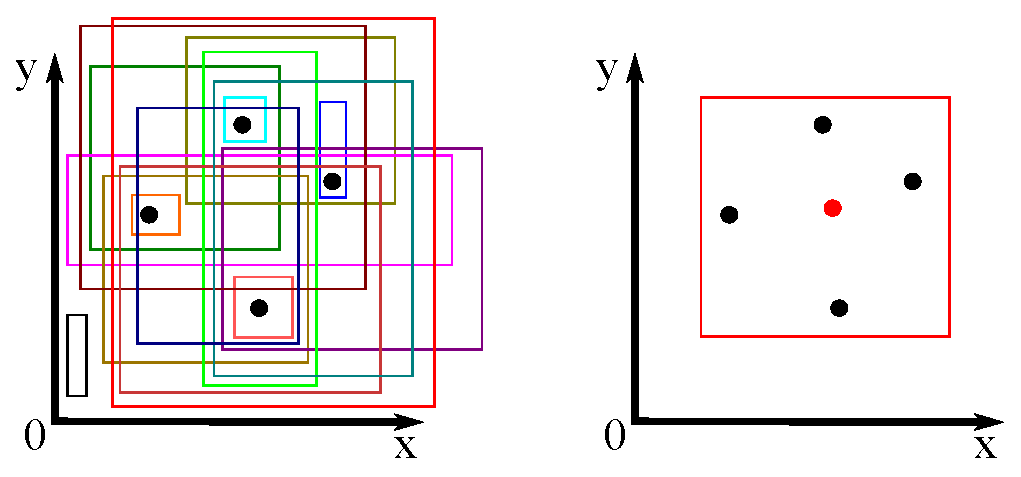
\includegraphics[width=.5\textwidth,keepaspectratio]{rectangles}
  \caption{Example of range space and VC-dimension. The space of points is the
  plane $\mathbb{R}^2$ and the set of ranges is the set of all
  \emph{axis-aligned rectangles}. The figure on the left shows graphically that
  it is possible to shatter a set of four points using 16 rectangles. On the
  right instead, one can see that it is impossible to shatter five points, as,
  for any choice of the five points, there will always be one (the red point in
  the figure) that is internal to the convex hull of the other four, so it would
  be impossible to find an axis-aligned rectangle containing the four points
  but not the internal one. Hence $\VC((X,R))=4$.}
  \label{fig:rectangles}
\end{figure}
%\begin{lemma}\label{lem:matousek}
%  The VC-Dimension of the range space $(\mathbb{R}^d, X)$, where $X$ is the set
%  of all half-spaces in $\mathbb{R}^d$ equals $d+1$.
%\end{lemma}

The main application of VC-dimension in statistics and learning theory is its
relation to the size of the sample needed to approximate learning the ranges, in
the following sense.

\begin{definition}\label{defn:eapprox}
  Let $(X,R)$ be a range space and let $A$
  be a finite subset of $X$. For $0<\varepsilon<1$, a subset $B\subset A$ is an
  $\varepsilon${\em-approximation} for $A$ if for all $r\in R$, we have
      \begin{equation}\label{eq:defeapprox}
	\left|\frac{|A\cap r|}{|A|}-\frac{|B\cap r|}{|B|}\right| \leq
	\varepsilon.
      \end{equation}
\end{definition}

%A similar definition offers relative guarantees.
%\begin{definition}\label{defn:releapprox}
%  Let $(X,R)$ be a range space and let $A$
%  be a finite subset of $X$. For $0<p,\varepsilon<1$, a subset $B\subset A$ is a
%  \emph{relative} $(p,\varepsilon)$\emph{-approximation} for $A$ if for any
%  range $r\in R$ such that $|A\cap r|/|A|\geq p$ we have 
%  \[ \left|\frac{|A\cap r|}{|A|}-\frac{|B\cap r|}{|B|}\right| \leq
%  \varepsilon\frac{|A\cap r|}{|A|}
%  \]
%  and for any range $r\in R$ such that $|A\cap r|/|A|< p$ we have $|B\cap
%	r|/|B| \leq (1+\varepsilon)p$.
%\end{definition}
%
An $\varepsilon$-approximation can be constructed by random sampling points of
the domain~[\citealp{HarPS11}, Thm.~2.12, see also~\citep{LiLS01}].

\begin{theorem}\label{thm:eapprox}
  There is an absolute positive constant $c$
  such that if $(X,R)$ is a range-space of VC-dimension at most $v$, $A\subset
  X$ is a finite subset and $0<\varepsilon,\delta<1$, then a
  random subset $B\subset A$ of cardinality $m$, where
  \begin{equation}\label{eq:eapprox}
    m\ge\min\left\{|A|,\frac{c}{\varepsilon^2}\left(v+\log\frac{1}{\delta}\right)\right\},
  \end{equation}
  is an $\varepsilon$-approximation for $A$ with probability at least $1-\delta$.
\end{theorem}

Note that throughout the work we assume the sample to be drawn \emph{with}
replacement if $m<|A|$, otherwise the sample is exactly the set $A$. The
constant $c$ is absolute and does not depend on the range space or on
any other parameter. \citet{LofflerP09} %showed 
estimated experimentally that the absolute constant $c$ is at most $0.5$. Up to
a constant, the bound presented in Thm.~\ref{thm:eapprox} is tight~\citep[Thm.~5]{LiLS01}. 

It is also interesting to note that an $\varepsilon$-approximation of size
$O(v\varepsilon^{-2}(\log v-\log\varepsilon))$ can be built
\emph{deterministically} in time
$O(v^{3v}(\varepsilon^{-2}(\log v-\log\varepsilon))^v|X|)$~\citep{Chazelle00}.

